%---------------------------------------------------------------------------------
\chapter{Introduction}
\label{chap:introduction}
%---------------------------------------------------------------------------------

%============================================== Background
\section{Background}
Recently, diffusion models \cite{nips_ddpm} \cite{iclr_ddim} \cite{lu2022dpm} have broken the leading performance of Generative Adversarial Networks (GANs) \cite{NIPS2014_5ca3e9b1} on image generation task and become the new state-of-the-art deep generative models. 
They have drawn great attention of AI researchers and have been rapidly applied to various generation tasks, such as image \cite{highresLDM}\cite{diff_autoencoder}, video\cite{videoDM}, audio\cite{oord2016wavenet}, natural language\cite{brown2020language} and multimodality \cite{url_stable} \cite{url_dalle2} \cite{cvpr_tcig}. 
Essentially, diffusion models consist of two processes: forward process and reverse process. In the forward process, a sample $x_0$ is perturbed into $x_T$ by progressively injecting Gaussian noise from time step $t=0$ to $t=T$, where $x_T$ becomes approximate pure noise and loses all structure of $x_0$. In the reverse process, starting from Gaussian noise $x_T$, diffusion models learn to denoise the data gradually until $t=0$, arriving at a new sample. Since the reverse process is to generate samples, it is also called sampling process. 
Unlike other generative counterparts such as GANs, variational autoencoders (VAE)\cite{kingma2013auto}, autoregressive models\cite{van2016conditional} and normalizing flows \cite{kingma2018glow} \cite{rezende2015variational} whose generation process is only one-time pass, diffusion models demand multiple iterative steps to generate sample.

Ideally, diffusion sampling process should be continuous and the step count $T\rightarrow\infty$. This would be convenient for mathematical modeling and analysis \cite{song2020score}.
But in practice sampling process is discretized and $T$ is assigned a reasonable value, such as $T=1000$ in paper \cite{nips_ddpm}. Such discretization will cause error because the discretized trajectory will deviate from the continuous one. Meanwhile, diffusion models themselves also have prediction error: the mismatch between predicted noise (or $x_0$) and the ground truth. And such prediction error will cause fitting error in sampling process.
As elaborated in paper \cite{zhang2022deis}, both of the discretization error and fitting error will thwart the sampling quality. That is illustrated in Fig \ref{fig:error-d-vs-p}.
% So there is dilemma when discretizing the sampling trajectory: more steps mean closer to ground truth trajectory, but slower in generation; and vice versa.

\begin{figure}[t] 
\centering
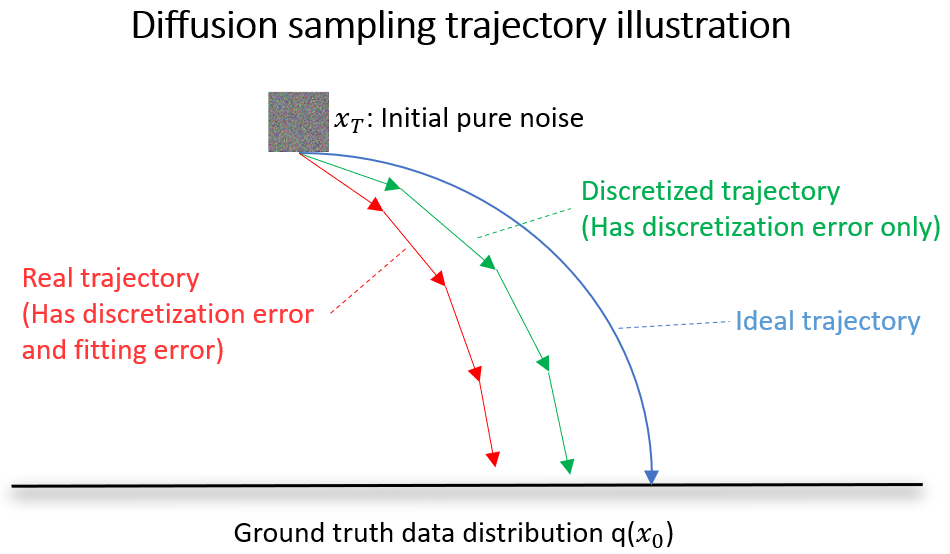
\includegraphics[width=0.45\textwidth]{figure/Error_discretization_vs_prediction.png}
\caption{Sampling trajectory illustration. In diffusion sampling process, there are two kinds of error: discretization error and fitting error. 
    The former happens when discretizing sampling process; and the latter is due to the mismatch between prediction and ground truth.}
\label{fig:error-d-vs-p}
\end{figure}

%============================================== Motivations
\section{Motivations}
Originally, diffusion sampling process needs hundreds or even thousands of steps, which is time-consuming and far from real-world requirements. The solution is fast sampling with fewer steps.
For this purpose, various approaches have been proposed to mitigate the discretization error. Yang Song used SDE in \cite{song2020score}; Lu Cheng adopted ODE in \cite{lu2022dpm}; and Luping Liu proposed numerical methods in \cite{liu2022pndm}, including linear multi-step, Runge Kutta\cite{runge_kutta} and so on. However, most of the prior works are focusing on the discretization error, but ignorant of the fitting error.
This motivates us a question: is it possible to reduce the impact of fitting error? More specifically, if a diffusion model is well-trained and sampling trajectory is pre-defined, is it possible to optimize the trajectory so as to reduce the influence of fitting error?

Of that question, one important prerequisite is that we won't re-train the model. And in fact, large models are difficult to re-train. One example is Stable Diffusion \cite{url_dpm} model. It was obtained by training on 4000 A100 GPUs with 5.9B image-text instances for one month. It would be hard for individuals or small institute to handle it. And possibly there will be larger and more complicated models in the future.

For that question, this study proposes a new problem setting: given a well-trained diffusion model $\theta(x_t, t)$ and a sampling trajectory with K steps $\{\bar{\alpha}_t|t=1, \cdots, K\}$ (where $0<\bar{\alpha}_t< 1$ controls the proportion of $x_0$ in $x_t$), how to improve the trajectory so as to improve sampling quality. 
Figure \ref{fig:compare-ab-img} gives an example: original trajectory and improved trajectory have the same step count but different step size; meanwhile the improved trajectory has much better sample result than the original one.

\begin{figure*} 
\centering
\begin{minipage}[h]{\textwidth}
  \subcaptionbox{$\bar{\alpha}$ values \label{fig:compare-ab-img-a}}
  {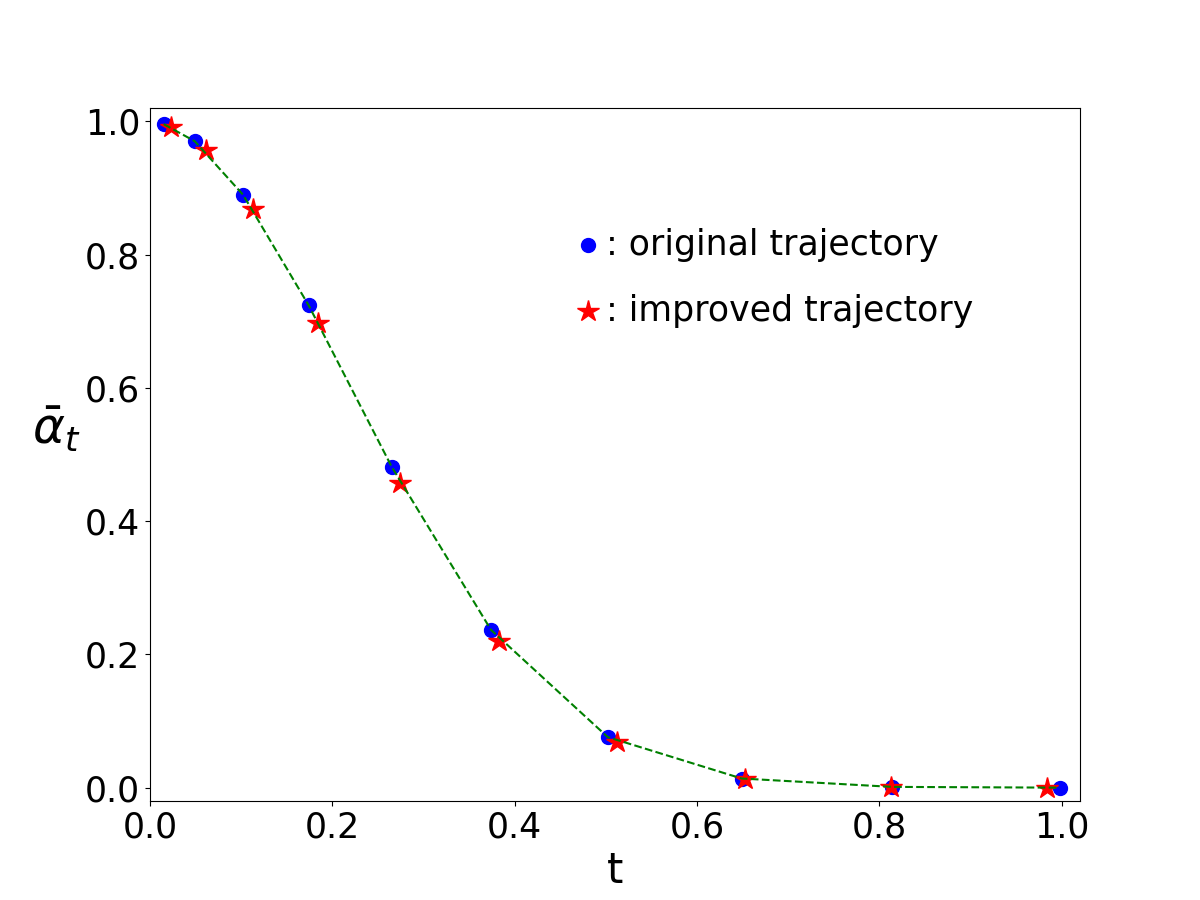
\includegraphics[width=.3\textwidth]{figure/abc_o2_s10_tq.png}}
  \subcaptionbox{Generated images. \label{fig:compare-ab-img-b}}
  {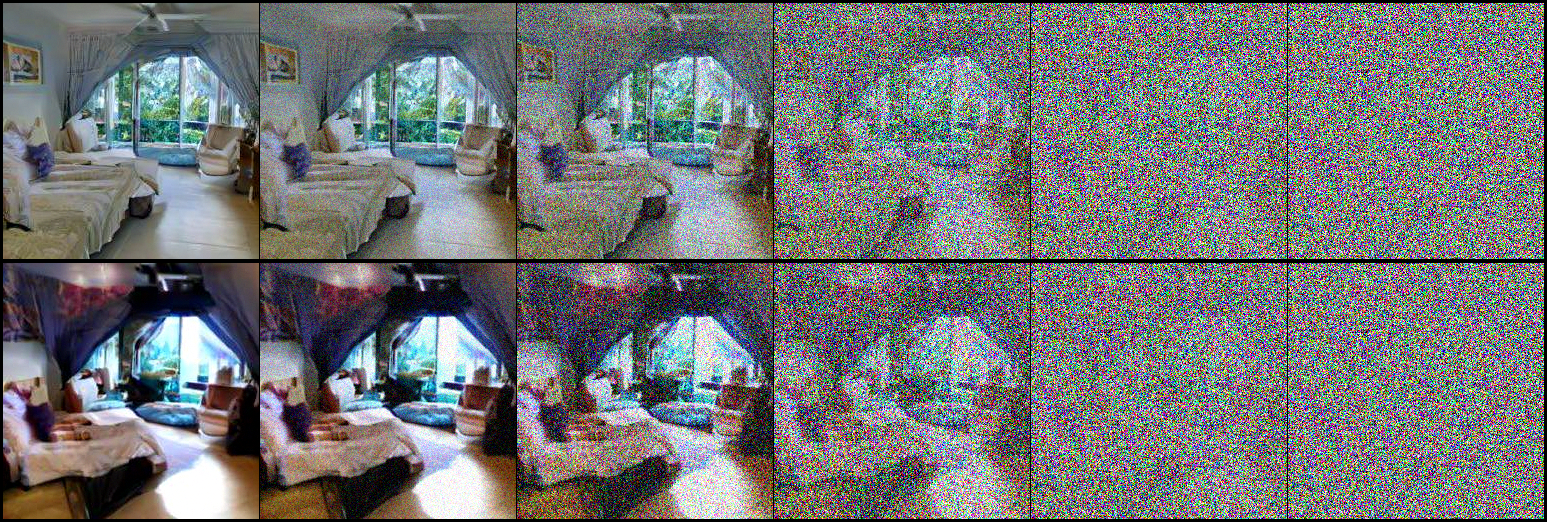
\includegraphics[width=.6\textwidth]{figure/bedroom-compare-with-inter-steps.png}}
\caption{Sampling trajectory and generated images of LSUN-bedroom\cite{url_dset_lsun-bedroom}. 
  The backbone sampler is DPM-Solver\cite{lu2022dpm} with order=$2$, schedule=\textit{quadratic} and steps=$10$.
  (a) $\bar{\alpha}$ values of original trajectory (blue dots) and improved trajectory (red stars). The horizontal axis is time step $t$ and the vertical axis is $\bar{\alpha}$ value. 
  (b) row 1: Image generated by improved trajectory. row 2: image generated by original trajectory. Both images are sampled from identical noise with the same step count. From left to right, the step indices are 0, 2, 4, 6, 8, 10. Notes: step 0 means the final generated image and step 10 means the initial noise.} 
\label{fig:compare-ab-img}
\end{minipage}
\end{figure*}

%============================================== Objective of Work
\section{Objective of Work}
To search for a better sampling trajectory, this paper proposes to track diffusion model's prediction error during sampling process, and then evaluate and reduce the impact of such error. Based on that idea, it introduces a quantitative method --- Variance-reduction Guidance (VRG) --- to help navigating the searching direction. In implementation, it designs an ingenious neural network to optimize the trajectory by minimizing VRG via standard SGD optimization.
% ingenious is_from: 59 Stochastic Trajectory Prediction via Motion Indeterminacy Diffusion
Comprehensive experiments demonstrate that decreasing the VRG value will get better sampling trajectory and improve generation quality. VRG method is training-free and model agnostic. It can be used in discrete-time and continuous-time diffusion models, and works well in conditional and unconditional generation tasks. 
% Moreover, given a pre-trained model, it only optimizes the step size in trajectory and won't bring any burden in sampling process.

Prediction error has big impact on sampling quality and such impact can be reduced by optimizing sampling trajectory. 
To the best of our knowledge, such relationship has not been revealed in prior work of diffusion models.
% sentence is_from: 74 DPM-Solver: A Fast ODE Solver for Diffusion Probabilistic Model Sampling in Around 10 Steps
% "To the best of our knowledge, such formulation has not been revealed in prior work of diffusion models."
This paper sheds a new light on diffusion model fast sampling and the main contributions are highlighted as below:

\begin{itemize}
 \item introduce a new problem setting about the impact of prediction error.
 % \item how to find better trajectory for off-the-shelf models.
 \item find a formulation to measure the prediction error impact.
 \item propose Variance-reduction Guidance method and solve its optimization problem by neural network.
 \item apply the proposed method to state-of-the-art works and verify its efficacy by experiments.
\end{itemize}
 
 %============================================== Report Outline
% \section{Report Outline}

% The remaining part of this report is organized as follows.

% The state-of-the-art and suitable spectral efficiency techniques for aeronautical communications are discussed in Chapter II. In particular, future candidate technologies for various flight domains in aeronautical communications are presented as part of the state-of-the-art. Studies on aeronautical channel modeling are then presented, before further discussions on suitable spectral efficiency techniques for aeronautical communications 

% In Chapter III, improvements to aeronautical waveforms over aeronautical communication channels are discussed. In particular, a new modulation scheme is proposed, simulated and compared, over various fading environments, against existing modulation schemes used in aeronautical communications.

% Discussions on a proposed HBD system for aeronautical communications are presented in Chapter IV. The performance of the proposed HBD system is evaluated from both the outage probability and finite SNR DMT perspective, and is compared against existing HD systems.

% Finally, future extensions of the works in Chapter III and Chapter IV are presented before the conclusion of this report in Chapter V.

%This report is organized as follows:
%
%Chapter 2 provides ....................................
%
%Chapter 3 reviews ....................................
%
%Chapter 4 discusses ....................................
%
%In Chapter 5, we propose ....................................
%
%Finally, we conclude in Chapter 6, where we also discuss about the
%directions and schedule of our future research.
